\documentclass[a4paper,12pt]{scrartcl}
\usepackage[a4paper,top=2.5cm,bottom=2.5cm,left=2cm,right=2cm]{geometry}
\usepackage{cmap,microtype}
\usepackage[utf8]{inputenc}
\usepackage[T1]{fontenc}
%\usepackage[scale=.87]{tgheros}
%\usepackage{tgtermes}
%\usepackage[lite]{mtpro2}
\usepackage{libertine}
\renewcommand\ttdefault{txtt}
\usepackage[english]{babel}

\usepackage{relsize}
\usepackage[smallcaps]{glossaries}
\loadglsentries{acronymlist}

\usepackage{graphicx,paralist,tabularx,wasysym,multicol,textcomp}
\setlength\pltopsep{6pt}
\usepackage[x11names,dvipsnames,svgnames]{xcolor}
\usepackage[os=win]{menukeys}
\usepackage{listings}
\lstset{language=[LaTeX]TeX,columns=fullflexible,
basicstyle=\ttfamily,texcsstyle=*\bfseries\color{NavyBlue},
commentstyle=\itshape\color{PaleVioletRed4},
frame=single,framesep=6pt,
framexleftmargin=6pt,framexrightmargin=6pt,
xleftmargin=12pt,xrightmargin=12pt,
breaklines=true,breakatwhitespace=true}

\usepackage{hyperref,cleveref}
\usepackage{apacite}
\bibliographystyle{apacite}


\title{Guide on Using umalayathesis}
\subtitle{version 1.2}
\author{Lim Lian Tze\\\texttt{\smaller liantze\string@gmail.com}}
\date{\smaller May 16, 2016}
\begin{document}
\maketitle

%\begin{center}
%\setlength\fboxsep{12pt}
%\fbox{\begin{minipage}{.7\textwidth}
%\noindent\emph{\textbf{Disclaimer:} %This particular version of the guide was written \emph{very} quickly. Sorry if you find parts of it incoherent; I hope to improve it in the near future. Before then, e-mail me if you have any questions.}
%
%\noindent\emph{(I am \emph{not} a student at \textsc{um}: I developed \texttt{umalayathesis} as a favour for a friend who is a PhD candidate there.)}

%\medskip
%
%\noindent\emph{\textbf{\color{red}CAUTION:} The Thesis Preparation Guide did \emph{not} provide a sample Original Literary Work Declaration statement, and we have yet to get one from the IGS office despite several e-mails. \texttt{umalayathesis} generates a draft sample as a temporary measure. If you have any information on how the declaration should read/look like, please contact me!}
%\end{minipage}}
%\end{center}
%
%\bigskip

\textsf{umalayathesis} is a \LaTeX\ class for authoring theses that fulfil formatting specifications required by \gls{UM}, Malaysia. The thesis preparation guide can be accessed at \url{http://bit.ly/1WzW7kS}. 
%http://cmsad.um.edu.my/index1.php?pfct=ips&modul=Current_Students&pilihan=Rules_and_Regulations

A sample \texttt{thesis.tex} is included in the package, which I recommend you modify for your own thesis write-up. (You can rename it, but I'll stick with the file name `\texttt{thesis.tex}' throughout this guide.)

\section{Before You Start}
\subsection{Pre-requisite Packages}
To streamline things, install the following packages first before using \textsf{umalayathesis} or compiling the example \texttt{thesis.tex}:

\begin{minipage}{.8\textwidth}
\begin{multicols}{3}
\begin{compactitem}
\item \textsf{memoir}
\item \textsf{apacite}
%\item \textsf{multibib}
%\item \textsf{relsize}
%\item \textsf{endnotes}
\item \textsf{glossaries}
\item \textsf{babel}
\item \textsf{longtable}
\item \textsf{hyperref}
\item \textsf{xfor}
\item \textsf{etoolbox}
\item \textsf{paralist}
\item \textsf{lipsum} (for \texttt{thesis.tex} only)\raggedright
\end{compactitem}
\end{multicols}
\end{minipage}


\subsection{Files}\label{sec:files}
Here's a quick list of the files required when writing your thesis with the \textsf{umalayathesis} class. Easiest way to go about things is to put all the files in the same directory. (See \Cref{sec:howto} for more details.)
%
\begin{itemize}
\item \texttt{\bfseries umalayathesis.cls}, the \LaTeX\ class file implementing the \gls{UM} thesis formatting requirements.
\item A ``main driver'' \texttt{.tex} file of your thesis, analogous to \lstinline|int main()| or \lstinline|public static void main(String[])|. You can name this file anything you like; it is known as \texttt{thesis.tex} in this guide. (See \Cref{sec:howto}.) \par\textbf{This is the \emph{only} file that you should run the processing tools on!}
\item A \texttt{.tex} file containing your thesis abstract. (See \Cref{sec:abstract}.)
\item \texttt{.tex} files containing your thesis chapters and appendices, one chapter per file. (See \Cref{sec:chapters} and \Cref{sec:appendices}.)
\item A \texttt{.bib} file containing your references and  publications. (See \Cref{sec:bibliography}).
\item A \texttt{.tex} file containing your glossary. (See \Cref{sec:glossary}).
\end{itemize}

\subsection{TeXworks Configuration}\label{sec:texworks}
Assuming \textsf{TeXworks} is your \LaTeX\ editor of choice on Windows, you will probably want to configure it so that you can process your glossary and list of own publications from within \textsf{TeXworks}.

(You can always, of course, opt to run the relevant commands from the command line prompt, or adapt these configurations for other editors and operating systems: I have tested on Windows XP, Ubuntu and Mac OS X.)

\subsubsection{Tool Configuration for Generating the Glossary}\label{sec:texworks:makeglossaries}
Access the \textsf{TeXworks} menu \textsf{Edit $\triangleright$ Preferences\ldots\ $\triangleright$ Typesetting}. Add a new processing tool called ``\textsf{MakeGlossaries}''. Configure it as shown below:

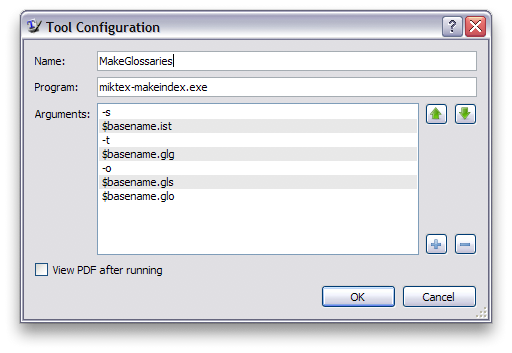
\includegraphics[width=.9\textwidth]{texworks-win_glossaries}

Now \textbf{repeat the above step} for another similar tool called ``\textsf{MakeAcronyms}'', but replace \texttt{``thesis.glg''} with \texttt{``thesis.alg''}; \texttt{``thesis.gls''} with \texttt{``thesis.acr''}; \texttt{``thesis.glo''} with \texttt{``thesis.acn''}.

On Linux and Mac systems, these are equivalent to the command lines

\medskip

\hspace{1em}\texttt{makeindex -s \textlangle base\textrangle.ist -t \textlangle base\textrangle.glg -o \textlangle base\textrangle.gls \textlangle base\textrangle.glo}

\subsubsection{Tool Configuration for Generating the List of Publications}
Now add a new processing tool called ``\textsf{Create Own Publication List}'' (or some other name). Configure it as shown below:

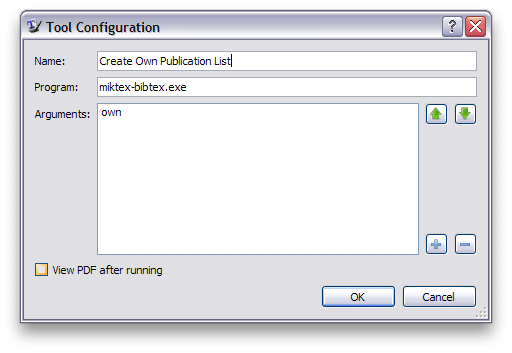
\includegraphics[width=.9\textwidth]{texworks-win_ownpub}


On Linux and Mac systems, these are equivalent to the command lines

\medskip

\hspace{1em}\texttt{bibtex own}


\subsubsection{Compiling \texttt{thesis.tex}}
The processing tools should be run on \texttt{thesis.tex} in the following sequence:
\begin{compactenum}
\item pdflatex + bibtex + makeindex
\item MakeGlossaries + MakeAcronyms + Create Own Publication List
\item pdflatex + bibtex + makeindex (twice)
\end{compactenum}

You will need to run `\textsf{MakeGlossaries}' and/or `\textsf{MakeAcronyms}' again if you add and use a \emph{new glossary entry}.

%\subsection{Why is there a blank page before the title page and at the end?!}
%The thesis preparation guidelines say there needs to be a blank page between the cover and the title page, and another at the very end, so \textsf{umalayathesis} forces one just in case you forgot to insert one. \texttt{;-)}

\subsection{Printing from Acrobat Reader}
Remember to set the \textbf{paper size} to \textbf{A4} and \textbf{page scaling} to \textbf{None} in the \textsf{Print} dialog, otherwise the margins would be incorrect.

\section{Using the umalayathesis Class}\label{sec:howto}

\subsection{Activation}\label{sec:activation}
To `activate' the class, make sure your main document file (e.g.\ \texttt{thesis.tex}) starts off with\\\lstinline|\documentclass{umthesis}|:

\medskip%\enlargethispage{\baselineskip}

\begin{lstlisting}
\documentclass{umalayathesis}
\usepackage{graphicx}
\usepackage{... other packages you need}
\end{lstlisting}

\medskip

This will set up the page margins, paragraph spacing, indents, page numbers, font face and size, citation and bibliography format, amongst other things. 

\subsection{Author Information}\label{sec:author:info}
You need to provide some author information in the preamble. Example lines from \texttt{thesis.tex}:

\medskip

\begin{lstlisting}[moretexcs={submissionyear,submissionmonth,faculty,degree,qualification}]
\author{Lim Lian Tze}
\title{My Ground-breaking Research}
\submissionyear{2012}
\faculty{Faculty of Amazing Research}
\degree{Doctor of Philosophy)}
\end{lstlisting}

\medskip

These information are needed to generate the preliminary pages.

\subsection{Preliminary Pages}\label{sec:prelim:pages}
Once in the main document body, \lstinline[moretexcs={frontmatter}]|\frontmatter| sets up the, well, front matter. This include setting the page numbers to lower-case Roman numerals.

\textsf{umalayathesis} can generate the cover page, title page and original literary work declaration page with the following lines (included in \texttt{thesis.tex}):

\medskip

\begin{lstlisting}[moretexcs={makecoverandtitlepage,copyrightpage,declarationpage}]
% \makecoverandtitlepage{\mastercoursework}
% \makecoverandtitlepage{\mastermixedmode}
% \makecoverandtitlepage{\masterresearch}
\makecoverandtitlepage{\doctoralresearch}
% \makecoverandtitlepage{\doctoralmixedmode}
\declarationpage
\end{lstlisting}

Please \emph{uncomment} the correct \lstinline|\makecoverandtitle| line to generate the correct statement on the title page.

\subsection{Acknowledgements}\label{sec:acknowledge}
\lstset{moretexcs={acknowledgements}}
This is provided using \lstinline|\acknowledgements|:

\medskip

\begin{lstlisting}
\acknowledgements{I would like to thank my parents, my family, my supervisor...}
\end{lstlisting}

\subsection{Abstract}\label{sec:abstract}
Write your abstracts in separate files (\texttt{sample-abstract.tex} for the English abstract and \texttt{sample-msabstract.tex} for the Malay abstract in this example), and include them in \texttt{thesis.tex} like this:

\begin{lstlisting}[moretexcs={abstractfromfile}]
\abstractfromfile{sample-abstract}
\msabstractfromfile{sample-msabstract}
\end{lstlisting}

\subsection{Table of contents, List of figures and tables}\label{sec:toc}

These are auto-generated by the following lines (included in \texttt{thesis.tex}):

\begin{lstlisting}[moretexcs={SingleSpacing,tableofcontents,listoftables,listoffigures}]
{\clearpage\SingleSpacing
\tableofcontents\clearpage
\listoffigures\clearpage
\listoftables\clearpage}
\end{lstlisting}


\subsection{Main Chapters}\label{sec:chapters}

I highly recommend that each chapter be written in a separate file. For example, \texttt{chap-intro.tex} has the contents

\begin{lstlisting}[moretexcs={chapter}]
%!TEX ROOT=thesis.tex
\chapter{Introduction}
This is the introduction chapter.

\section{Problem Background}
We study the...
\end{lstlisting}

\bigskip

And \texttt{chap-litreview.tex}:
\begin{lstlisting}[moretexcs={chapter}]
%!TEX ROOT=thesis.tex
\chapter{Literature Review}
We review the state of the art in...

\section{Early Approach}
Researchers first attempted to...
\end{lstlisting}

\bigskip

In \texttt{thesis.tex}, these chapter files are included with the following lines:
\begin{lstlisting}[keepspaces=true,moretexcs=mainmatter]
\mainmatter               % signal start of main chapters
\input{chap-intro}      % no .tex extension!
\input{chap-litreview}
\input{...}
\end{lstlisting}

\bigskip

The \lstinline|%!TEX ROOT=thesis.tex| indicates to \textsf{TeXworks} (and also \textsf{TeXshop} on the Mac) that \texttt{chap-xxx.tex} are `sub-files' of \texttt{thesis.tex}. This means if you hit \keys{Ctrl+T} when you  are editing \texttt{chap-xxx.tex}, \texttt{thesis.tex} will get compiled instead. Neat eh?

\subsection{Appendices}\label{sec:appendices}
Again, I recommend keeping each appendix chapter in its own file e.g.~\texttt{app-umldiagram.tex}:

\begin{lstlisting}
%!TEX ROOT=thesis.tex
\chapter{UML Diagrams}
...
\end{lstlisting}

\bigskip

And in \texttt{thesis.tex}:
\begin{lstlisting}[keepspaces=true,moretexcs={appendix}]
\appendix   % signal start of appendices
\input{app-umldiagram}
\input{...}
\end{lstlisting}


\subsection{Citations and Bibliography}\label{sec:bibliography}
\textsf{umalayathesis} uses the \textsf{apacite} package to format citations and bibliography in the APA style.

Here are some useful variants of the \lstinline|\cite| command; see the \textsf{apacite} manual for full list.

\bigskip

{\lstset{moretexcs={citeNP,citeauthor,citeyear}}
\begin{tabular}{>{\textbullet\hspace{6pt}}l @{\hspace{6pt}$\rightarrow$\hspace{6pt}} l}
\lstinline|\cite{Lim:2009}| & (Lim, 2009)\\
\lstinline|\citeNP{Lim:2009}| & Lim, 2009 (no parenthesis)\\
\lstinline|\cite<see>[p.~7]{Lim:2009}| & (see Lim, 2009, p.~7)\\
\lstinline|\citeauthor{Lim:2009}| & Lim\\
\lstinline|\citeyear{Lim:2009}| & (2009)\\
\end{tabular}
}

\bigskip

In \texttt{thesis.tex}, these lines will print the bibliography list:
\medskip
\begin{lstlisting}[keepspaces=true,moretexcs=backmatter]
\backmatter            % signal start of back matter
\bibliography{bibfile} % bibliography file name without .bib extension
\end{lstlisting}


\subsection{List of Publications}

First, make sure that you enter details about your own publications in your \verb|.bib| file.  Then in \verb|thesis.tex|, search for the following line:

\lstset{escapechar={}}
\begin{lstlisting}
\nociteown{Lim:2009}
\end{lstlisting}

Replace the BibTeX key between the curly braces with that of your own publication.  If you have more than one publications, simply separate them with commas inside the curly braces, like this:

\begin{lstlisting}
\nociteown{lim:tang:2004,Lim:2009}
\end{lstlisting}

If you add more publications to \verb|\nociteown| later, you will need to run \textsf{pdflatex} and the \textsf{Create Own Publication List} tool that you configured earlier, then 2 more runs of \textsf{pdflatex} for the list to appear properly.



\subsection{Glossary}\label{sec:glossary}
You can maintain a consistent glossary and acronym list using the \textsf{glossaries} package. It also supports acronym expansion on first mention! {\large\smiley}

First, define your acronyms and terms in a separate file e.g.~\texttt{myacronyms.tex}:

\medskip

\begin{lstlisting}[moretexcs={newacronym,newglossaryentry},basicstyle=\ttfamily\small,
emph={name,description,plural,firstplural},emphstyle=\bfseries]
% \newglossaryentry{label}{name={term},description={explanation}}
\newglossaryentry{lexicon}{
name={lexicon},
description={The vocabulary of a language, including its words and expressions. More formally, it is a language's inventory of lexemes}
}

% \newacronym[description={explanation}]{label}{abbrv}{full form}
\newacronym
[description={single word or words that are grouped in a language's lexicon}]
{LI}{LI}{lexical item}

\newacronym[description={The application of computational linguistics principles to problems}]
{NLP}{NLP}{Natural Language Processing}

% when the plural form is irregular, specify firstplural and plural
\newacronym
[firstplural={parts of speech}, plural={POS},
description={linguistic category of lexical items}]
{POS}{POS}{part of speech}
\end{lstlisting}

\bigskip

Loading the glossary and acronym list, and later printing the list of acronyms and glossary in \texttt{thesis.tex}:

\medskip

\begin{lstlisting}[moretexcs={loadglsentries,printglossaries,listofacronyms}]
% Must be loaded BEFORE \begin{document}!
\loadglsentries{myacronyms}
\begin{document}
...
% List of acronyms is between list of tables and list of appendices
\listofacronyms\clearpage
...
\bibliography{bibfile}
% Glossaries is placed AFTER the bibliography
% (only entries that are actually used in the text will be listed)
\printglossary
...
\end{lstlisting}

\bigskip

To mention them in the text (i.e.~\texttt{chap-xxx.tex} etc):

\medskip

\lstset{moretexcs={gls,glsplural,ac,acp,Gls,Glsplural,Ac,Acp}}
\begin{lstlisting}
Let's talk about \acp{LI} and \acp{POS} in \ac{NLP}. I mention again \acp{LI}. We will also talk about \glsplural{lexicon}.
\end{lstlisting}

\bigskip

Notice how the acronyms are expanded on first use, as well as the use of \lstinline|\glsplural| and \lstinline|\acp| for plurals:

\medskip

\fboxsep=12pt
\noindent\fbox{\begin{minipage}{.95\textwidth}
Let's talk about lexical items (LIs) and parts of speech (POS) in Natural 
Language Processing (NLP). I mention again LIs. We will also talk about lexicons. 
\end{minipage}}

\bigskip

You will need to run \textsf{pdflatex}, the \textsf{MakeGlossaries} and \textsf{MakeAcronyms} tool that you configured earlier, then 2 more runs of \textsf{pdflatex} for the glossaries to appear properly.

Use \lstinline|\Gls|, \lstinline|\Glsplural|, \lstinline|\Ac|, \lstinline|\Acp| etc.~if you need to capitalise the first letter of your terms at the beginning of sentences.

\end{document}
